\chapter{Backscatter Communication}
\label{ch:backscatter}

\begin{defbox}[In this chapter you will learn]
\begin{itemize}
 \item why a backscatter radio consumes microwatts where a conventional radio consumes milliwatts;
 \item how switching an antenna's load \emph{modulates} a reflection, using the reflection coefficient;
 \item how to derive the \emph{two-way} (radar-like) link budget and why its exponent doubles---exactly the formula behind Amber's uplink;
 \item the power-split trade-off between harvesting and reflecting, parameterised by $\eta$;
 \item why strong carrier self-interference forces \emph{frequency-shifted} backscatter, how a square-wave switch creates sidebands, and what Amber's \emph{subcarrier shifts} abstract;
 \item how a device with no receiver chain can still receive commands, and what the paper's dual-tone PRDCH idea contributes.
\end{itemize}
\end{defbox}

\section{Active radio versus backscatter radio}
\label{sec:activevsbs}

A conventional radio transmitter must \emph{create} a carrier. A crystal oscillator
sets the reference, a phase-locked loop multiplies it to the carrier
frequency, a mixer imposes the data, and a power amplifier raises the signal to
the level the link budget requires. Each block draws power; the amplifier alone,
at a typical efficiency of tens of percent, makes transmission cost on the order of
tens to hundreds of milliwatts for a wide-area link.

A \emph{backscatter} transmitter does none of that. It does not create RF
energy at all. It relies on an \emph{external source}---in our case the base
station's carrier---and changes how its own antenna \emph{reflects} the wave that
arrives. The only active element is a switch (a transistor) and the logic that
drives it, which can run on microwatts. The price is that
\begin{itemize}
 \item the transmit power is only a fraction of what the device received, so the uplink is weak (Section~\ref{sec:twoway});
 \item a strong external carrier must be present while the device talks;
 \item the reader's receiver must pick a faint reflection out of the carrier's own huge leakage (Section~\ref{sec:selfint}).
\end{itemize}
\begin{keyidea}
Backscatter trades \emph{device energy} for \emph{infrastructure complexity}: it moves the expensive parts of a radio (oscillator, mixer, amplifier) from the many cheap devices to the few base stations.
\end{keyidea}

\section{Modulating a reflection}
\label{sec:reflection}

Consider an antenna with complex impedance $Z_a$ terminated by a load $Z_L$. An
incident wave delivers power to the load unless the load reflects it. The
(power-wave) \emph{reflection coefficient} at the antenna terminals is
\begin{equation}
 \Gamma \;=\; \frac{Z_L-Z_a^{*}}{Z_L+Z_a}.
\label{eq:gamma}
\end{equation}
Two extremes capture the idea \citep{pozar2011,dobkin2012}.
\begin{itemize}
 \item \textbf{Absorbing (matched) state:} $Z_L=Z_a^{*}$ gives $\Gamma=0$. All captured
   power enters the load and can be \emph{rectified for harvesting}.
 \item \textbf{Reflecting state:} $Z_L=0$ (short) or $Z_L=\infty$ (open) gives
   $|\Gamma|=1$. The captured power is re-radiated.
\end{itemize}
A transistor that switches the load between two states $\Gamma_0$ and $\Gamma_1$ therefore
\emph{modulates the amplitude (and/or phase) of the reflected wave}, which is
the incident carrier multiplied by $\Gamma(t)$. Switching between $\Gamma_0=0$ and
$|\Gamma_1|=1$ gives amplitude-shift keying (on--off keying); switching between $+1$ and
$-1$ gives binary phase-shift keying (compare the OOK/BPSK modulations that
3GPP's Release-19 summaries report for the uplink).

\begin{figure}[t]
\centering
\begin{tikzpicture}[x=1cm,y=1cm,>=Stealth]
 % antenna
 \draw[line width=1.1pt] (0,0) -- (0,1.5);
 \draw[line width=1.1pt] (-0.35,1.5) -- (0.35,1.5);
 \draw[line width=1.1pt] (-0.22,1.2) -- (0.22,1.2);
 \draw[line width=1.1pt] (0,0) -- (1.2,0);
 \node[lab,anchor=east] at (-0.45,1.4) {antenna $Z_a$};
 % switch
 \node[box,minimum width=1.5cm,draw=aorange,fill=lightorange] (sw) at (2.3,0) {switch};
 \draw[line width=1.1pt] (1.2,0) -- (sw.west);
 % two branches
 \node[box,minimum width=2.6cm,draw=agreen,fill=lightgreen] (abs) at (6.2,0.95) {matched load\\$\Gamma\approx0$: absorb};
 \node[box,minimum width=2.6cm,draw=ared,fill=lightred] (ref) at (6.2,-0.95) {short / open\\$|\Gamma|\approx1$: reflect};
 \draw[->] (sw.east) -- ++(0.5,0) |- (abs.west);
 \draw[->] (sw.east) -- ++(0.5,0) |- (ref.west);
 \node[box,draw=agreen] (rect) at (9.9,0.95) {rectifier\\$\to C$};
 \draw[->] (abs) -- (rect);
 \node[box,draw=ablue,fill=lightblue] (log) at (2.3,-1.9) {logic /\\data bits};
 \draw[->] (log) -- (sw);
 \node[lab,anchor=west,align=left] at (7.7,-0.95) {re-radiated wave\\$=\Gamma(t)\times$ incident};
\end{tikzpicture}
\caption{A backscatter front-end. A digital switch connects the antenna either to a matched path that feeds the rectifier (energy harvesting) or to a reflecting termination. The data bits control the switch and thereby impose themselves on the reflected carrier. There is no oscillator, mixer or power amplifier.}
\label{fig:bsfrontend}
\end{figure}

\section{The two-way link budget}
\label{sec:twoway}

The key difference to a conventional link: the signal travels over \emph{two}
hops, the forward hop (reader to tag) and the reverse hop (tag to reader). Apply
the Friis equation twice.

\paragraph{Forward hop.} The power captured by the tag is
$P_{\mathrm{tag}}=P_t\,G_t\,G_a\,L(d_1)$, where $G_a$ is the tag antenna gain and
$L(d_1)=(\lambda/4\pi d_1)^2$ in free space.

\paragraph{Re-radiation.} The tag re-radiates a fraction $\eta$ of that power (the
\emph{backscatter efficiency}): $P_{\mathrm{bs}}=\eta\,P_{\mathrm{tag}}$.

\paragraph{Reverse hop.} The reader receives
$P_r=P_{\mathrm{bs}}\,G_a\,G_r\,L(d_2)$. Combining,
\begin{equation}
 P_r \;=\; P_t\,G_t\,G_r\,G_a^{2}\;\eta\;L(d_1)\,L(d_2)
 \;\stackrel{\text{free space}}{=}\; \frac{P_t\,G_t\,G_r\,G_a^{2}\,\eta\,\lambda^{4}}{(4\pi)^{4}\,d_1^{2}\,d_2^{2}}.
\label{eq:dyadic}
\end{equation}
This is the \emph{dyadic backscatter channel}, a close cousin of the radar
equation. When the reader's transmit and receive antennas coincide (a \emph{monostatic}
reader), $d_1=d_2=d$ and
\[
 P_r\ \propto\ d^{-4}.
\]
\textbf{The path-loss exponent doubles.} In decibels,
\begin{equation}
 P_r\,[\mathrm{dBm}] = P_t + G_t + G_r + 2G_a + 10\log_{10}\eta - \mathrm{PL}(d_1)-\mathrm{PL}(d_2).
\label{eq:dyadicdb}
\end{equation}

\begin{keyidea}[Amber's uplink is Eq.~\eqref{eq:dyadicdb}]
The simulator does not have a special ``backscatter channel.'' It composes
two ordinary hops. \codew{calculate_node_power} stores the downlink power
multiplied by $\eta$ as the node's \codew{backscatter_power_dbm}; \codew{compute_point_to_bs}
then treats that as the \emph{transmit power} of a new link, multiplies it by
the node's antenna gain, applies the same path loss again, and multiplies by the sector's
receive gain. In decibels this is exactly Eq.~\eqref{eq:dyadicdb} with
$d_1=d_2$ (same sector, same node, same model). The hand calculation of
Chapter~\ref{ch:decibels} reproduced the logged $-45.71$~dBm to two decimals.
\end{keyidea}

\begin{figure}[t]
\centering
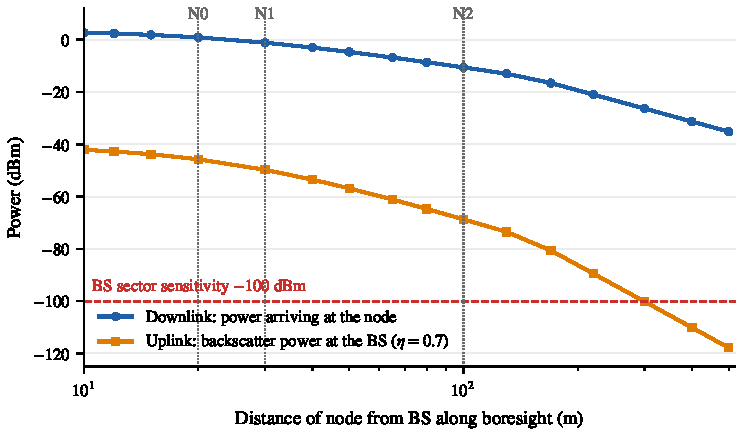
\includegraphics[width=0.88\linewidth]{fig_budget}
\caption{Downlink power at the node and uplink backscatter power at the base station against distance, for the demo's north-facing sector ($\SI{46}{dBm}$, $\SI{15}{dBi}$, $\eta=0.7$), computed by Amber. The uplink starts $\sim\SI{45}{dB}$ lower and falls twice as fast. With the demo's $\SI{-100}{dBm}$ sector sensitivity the link would close out to about $\SI{300}{m}$; the node would be energy-limited long before.}
\label{fig:budget}
\end{figure}

\paragraph{Which hop limits the system?}
A tag works only if \emph{both} conditions hold:
\begin{align*}
 &\text{(forward / energy)} && P_{\mathrm{tag}}\ \text{large enough to power the device,}\\
 &\text{(reverse / information)} && P_r\ge S_{\mathrm{rx}}.
\end{align*}
Which one fails first depends on design. For a passive tag with no storage, the
forward link usually limits: the rectifier needs of order $\SI{-20}{dBm}$ or more to
turn on. For a device with a battery or large storage the reverse
link limits. In Amber's demos the downlink is generous (milliwatts at $\le\SI{30}{m}$),
and the uplink margin at $\SI{100}{m}$ is over $30$~dB, so the energy
\emph{accumulation time} (Chapter~\ref{ch:capacitor}) rather than the link margin
decides how often a node can talk.

\begin{example}[The paper's scenario: can an RF-only node even start?]
The paper's experiment uses $\SI{30}{dBm}$ sectors with $\SI{17}{dBi}$, $\SI{1}{dBi}$ nodes and 924~MHz.
At $\SI{20}{m}$ the UMa LOS loss is $\SI{60.1}{dB}$, so the node receives
$30+17+1-60.1=\SI{-12.1}{dBm}=\SI{62}{\micro W}$; at $\SI{100}{m}$ only $\SI{-23.6}{dBm}=\SI{4.4}{\micro W}$.
Under Amber's harvesting model with the demo's $\Rs=\SI{5}{k\ohm}$ these correspond to
equivalent source voltages $\sqrt{P\Rs}\approx\SI{0.56}{V}$ and $\SI{0.15}{V}$
(Chapter~\ref{ch:harvest}), far below the $\Vhigh=\SI{1.7}{V}$ used in the demos.
Even the best case beyond $\SI{10}{m}$ gives only $\approx\SI{0.65}{V}$. \emph{Such
nodes can never wake up on RF alone}---which is why the paper operates them in
\textbf{hybrid power mode} with an external (solar) source. The thresholds and
$\Rs$ of the paper's run are not stated in the abstract; we use the demo values.
\end{example}

\section{Splitting power between harvesting and reflecting}
\label{sec:split}

An antenna captures a fixed amount of power. What it \emph{reflects} it
cannot also \emph{rectify}; to first order,
\[
 P_{\mathrm{harvest}} + P_{\mathrm{reflect}} = P_{\mathrm{captured}}.
\]
The paper describes nodes by ``a power split ratio determining how received RF
power is divided between energy harvesting and backscatter reflection.'' In Amber
that ratio is $\eta=$ \codew{Node.efficiency} $\in[0,1]$ (default~1), and the
bookkeeping is a \emph{state-dependent} one:
\begin{align}
 P_{\mathrm{backscatter}} &= \eta\,P_{\mathrm{dl}} && \text{(always computed)},\\
 P_{\mathrm{harvest}} &=
 \begin{cases}
  P_{\mathrm{dl}} & \text{node not transmitting},\\
  (1-\eta)\,P_{\mathrm{dl}} & \text{node in the \emph{transmitting} state.}
 \end{cases}
\end{align}
While the node is idle its antenna absorbs everything; while it
transmits a fraction $\eta$ is reflected and so lost to the harvester. Because
transmissions are brief this costs little energy, but the model captures the
principle that \emph{communicating and harvesting compete for the same photons}.
For Node~0 ($P_{\mathrm{dl}}=\SI{1.24}{mW}$, $\eta=0.7$) the equivalent
source voltage drops from $\SI{2.49}{V}$ to $\SI{1.36}{V}$ for the duration of a transmission.

\begin{reality}[What $\eta$ must absorb]
In Amber $\eta$ is a \emph{single scalar} that must stand for everything that
reduces the reflected \emph{information-bearing} power: the incomplete modulation depth,
the conversion of carrier power into the wanted sideband (next section),
the antenna's mismatch and structural scattering. A square-wave-shifted OOK
tag, for instance, puts only $(1/\pi)^2\approx0.10$ of the incident power into
each first sideband. The default $\eta=1$ is therefore the most optimistic choice;
the shipped demos use $0.7$. Choose it deliberately.
\end{reality}

\section{Self-interference and frequency-shifted backscatter}
\label{sec:selfint}

Recall the dynamic-range problem of Section~\ref{sec:dynrange}: the reader's own
carrier, even after $\sim\SI{25}{dB}$ of antenna isolation, is tens of dB stronger
than the reflected data. A receiver cannot filter it out if the wanted signal sits
at the \emph{same} frequency. The solution is to move the reply away
in frequency.

Let the incident carrier be $x(t)=A\cos(2\pi f_ct)$ and let the tag toggle its
reflection coefficient between $\Gamma_0$ and $\Gamma_1$ with a unit square wave
$s(t)\in\{0,1\}$ of frequency $f_s$, so that $\Gamma(t)=\Gamma_0+\Delta\Gamma\,s(t)$,
$\Delta\Gamma=\Gamma_1-\Gamma_0$. The Fourier series of the square wave is
$s(t)=\tfrac12+\tfrac{2}{\pi}\sum_{k\ \mathrm{odd}}\tfrac1k\sin(2\pi kf_st)$. The
reflected signal $y(t)=\Gamma(t)x(t)$ is therefore
\begin{align}
 y(t)&=\Big(\Gamma_0+\tfrac{\Delta\Gamma}{2}\Big)A\cos(2\pi f_ct)\label{eq:y0}\\
 &\quad+\frac{\Delta\Gamma}{\pi}A\Big[\sin\big(2\pi(f_c+f_s)t\big)-\sin\big(2\pi(f_c-f_s)t\big)\Big]+\text{odd harmonics}.\label{eq:y1}
\end{align}
Term~\eqref{eq:y0} is a copy of the carrier at $f_c$ (the
\emph{static} reflection, carrying no data). The information-bearing
energy appears at $f_c\pm f_s$ in \eqref{eq:y1}. Each first-order sideband has power
$(\Delta\Gamma/\pi)^2$ times the incident carrier power: for
$\Delta\Gamma=1$ (on--off) that is $-9.9$~dB; for a phase flip between $+1$ and
$-1$ ($\Delta\Gamma=2$) it is $-3.9$~dB. The reader now tunes its receiver to
$f_c+f_s$, where the carrier leakage is absent.

\begin{figure}[t]
\centering
\begin{tikzpicture}[x=1cm,y=1cm]
 \draw[->] (-1.0,0) -- (12.2,0) node[right,lab] {frequency};
 % carrier
 \draw[->,line width=2pt,ablue] (1.5,0) -- (1.5,3.0);
 \node[lab,ablue,align=center,anchor=south] at (1.5,3.05) {unmodulated carrier\\(dedicated subcarrier)};
 % downlink data subcarrier
 \draw[->,line width=2pt,agrey] (0.0,0) -- (0.0,1.5);
 \node[lab,agrey,align=center,anchor=south] at (-0.1,1.55) {data subcarrier\\(downlink commands)};
 % backscatter groups
 \foreach \x/\c/\n in {4.2/agreen/1,6.6/aorange/2,9.0/apurple/3}{
   \draw[->,line width=1.6pt,\c] (\x,0) -- (\x,0.55);
   \draw[->,line width=1.6pt,\c] (\x+0.3,0) -- (\x+0.3,0.4);
   \draw[->,line width=1.6pt,\c] (\x-0.3,0) -- (\x-0.3,0.4);
   \node[lab,\c,anchor=north] at (\x,-0.15) {shift $\n$};
 }
 \draw[<->,agrey] (1.5,-0.85) -- node[lab,below]{$f_{s,1}$} (4.2,-0.85);
 \draw[<->,agrey] (1.5,-1.35) -- node[lab,below]{$f_{s,2}$} (6.6,-1.35);
 \draw[<->,agrey] (1.5,-1.85) -- node[lab,below]{$f_{s,3}$} (9.0,-1.85);
 \node[lab,align=left,anchor=west] at (9.8,1.3) {\textcolor{agreen}{nodes in the same}\\\textcolor{agreen}{group share a shift:}\\\textcolor{agreen}{they can collide}\\and need SIC};
\end{tikzpicture}
\caption{Frequency-domain picture of the dual-tone downlink and frequency-shifted backscatter. A clean carrier on a dedicated subcarrier powers and illuminates the nodes; one data-bearing subcarrier carries the downlink. Each node reflects its reply at an offset $f_{s,k}$ from the carrier (shown on one side only; real sidebands appear on both). Different offsets are \emph{orthogonal}; nodes with the same offset overlap in frequency and time and must be separated by capture or SIC (Chapter~\ref{ch:sic}).}
\label{fig:spectrum}
\end{figure}

\paragraph{Frequency shifting as multiple access.}
If different nodes choose \emph{different} $f_s$, their replies land in different
frequency slots and do not collide even if they transmit simultaneously. The
paper's three \emph{subcarrier shifts} exploit exactly this: ``Distinct subcarrier
offsets provide frequency-domain separation, and successive interference
cancellation (SIC) resolves collisions among nodes sharing the same offset.''
Subcarrier shifting thus has \emph{two} roles: keeping replies away from carrier
interference, and acting as a coarse FDMA-style resource.

\begin{reality}[How Amber models subcarrier shifts]
Amber does not synthesise any spectrum. \codew{Node.subcarrier_shift} is an
\emph{integer label}; the base station groups packets by that label and
assumes that different labels are \emph{perfectly orthogonal}
(Chapter~\ref{ch:sic}). Neither carrier leakage, adjacent-shift leakage, nor the
sideband loss of Eq.~\eqref{eq:y1} is modelled explicitly---the latter is yours to place
inside $\eta$.
\end{reality}

\section{Receiving with no receiver: the passive downlink}
\label{sec:passivedl}

So far we have covered uplink. How does a $\mu$W device \emph{hear} commands?
A conventional receiver needs a low-noise amplifier, a local oscillator and a
mixer, and consumes milliwatts. A passive device instead uses an
\emph{envelope detector}: a diode followed by a low-pass filter that outputs
the slowly varying \emph{amplitude} of the incoming signal, much like a crystal
radio. It works naturally with \emph{on--off keying} (OOK): a ``1'' is
carrier present, a ``0'' is carrier absent. The 3GPP Release-19 summaries
describe exactly this: an RF envelope-detection receiver and OOK on the
reader-to-device link. The costs are poor sensitivity (typically in the region of
$\SI{-40}{dBm}$ to $\SI{-50}{dBm}$ for simple passive detectors, tens of dB
worse than an active receiver) and low data rates---which is why Amber's default
\emph{node} sensitivity is $\SI{-45}{dBm}$ while its \emph{sector} sensitivity
is $\SI{-100}{dBm}$.

\paragraph{OFDMA downlinks for passive nodes.}
Cellular networks use OFDM, whose many subcarriers are normally separated by
an FFT, which is expensive. The paper cites Zhu et al.\
\citep{zhu2022ofdma}, who demonstrate OFDMA downlink demodulation at around
$\SI{100}{\micro W}$ by replacing the digital FFT with \emph{analogue
filtering}. This is the enabling idea behind the Amber paper's \emph{dual-tone
principle}.

\paragraph{The dual-tone PRDCH.}
The paper says that Amber's physical layer is by default based on the
\emph{Physical Reader to Device Channel} (PRDCH): ``an external unmodulated
carrier occupies a dedicated OFDM subcarrier, enabling both energy harvesting
and backscatter reflection \citep{zhu2022ofdma}, while a single data-bearing
subcarrier carries downlink information from base station to node.'' Two tones,
two jobs:
\begin{enumerate}
 \item the \emph{carrier tone} is a clean sinusoid, ideal both for harvesting
   (constant, rectifier-friendly power) and as the illumination to be reflected
   (nothing to cancel except the carrier itself);
 \item the \emph{data subcarrier} carries OOK-like commands that an analogue
   filter can separate from the carrier.
\end{enumerate}
Figure~\ref{fig:spectrum} sketches this arrangement. In 3GPP's terms the
PRDCH is the physical reader-to-device channel studied in TR~38.769.

\begin{reality}[The downlink is not waveform-simulated]
In Amber a command is a Python call. It is delivered if the best downlink
power reaching the node exceeds the node's sensitivity; there are no bit errors,
no demodulation, no data-rate limit and no per-command energy cost to the
node. The \emph{carrier} is implicit and always on: the base-station behaviour
class states that nodes ``harvest energy all the time'' and that ``the schedule
only handles communication''.
\end{reality}

\section{Topologies and duplexing}

Literature distinguishes three backscatter arrangements \citep{huynh2018ambient}.
\begin{description}[leftmargin=0.5cm,font=\sffamily\bfseries]
 \item[Monostatic.] The reader transmits the carrier and receives the reflection
   (one device, or two collocated). The forward and return distances are equal,
   $P_r\propto d^{-4}$. This is Amber's arrangement.
 \item[Bistatic.] A separate \emph{carrier emitter} illuminates the tag while the
   receiver is elsewhere; $d_1\ne d_2$. This resembles 3GPP's topology~T3 (with an assisting node).
 \item[Ambient.] The carrier is an unrelated, already-present signal (TV,
   Wi-Fi, cellular \citep{liu2013ambient}); the tag has no control over it.
\end{description}
The paper describes the reference experiment as a polling protocol ``operating
in full-duplex mode''. Because the carrier is transmitted \emph{continuously} on
its own subcarrier, the base station can receive backscatter while the carrier
is on. Amber's \emph{schedule} nevertheless alternates TX (command) and RX
(reply) windows: the command is on the data subcarrier and the base station
does not listen while it sends one (Chapter~\ref{ch:bsengine}).

\begin{codemap}
\small
\begin{tabularx}{\linewidth}{@{}>{\ttfamily}p{5.6cm}X@{}}
\toprule
\normalfont\bfseries Concept & \normalfont\bfseries Code (\file{amber/})\\
\midrule
Backscatter / harvest split $\eta$ & \codew{CoverageMap.calculate_node_power}; \codew{Node.efficiency}\\
Dyadic uplink budget, Eq.~\eqref{eq:dyadicdb} & \codew{CoverageMap.compute_point_to_bs}\\
Subcarrier label & \codew{Node.subcarrier_shift}; \codew{BSBehavior._process_rx_buffer}\\
Command reception gate & \codew{BackscatterModule.receive_command}\\
Always-on carrier & documented in \code{BSBehavior}; no explicit object\\
\bottomrule
\end{tabularx}
\end{codemap}

\section{Chapter summary}
\begin{itemize}
 \item Backscatter saves energy by switching a reflection instead of generating a carrier; the switch alternates between absorbing ($\Gamma\approx0$) and reflecting ($|\Gamma|\approx1$).
 \item The dyadic link $P_r=P_tG_tG_rG_a^2\,\eta\,L(d_1)L(d_2)$ has a doubled path-loss exponent; Amber implements it as two chained hops.
 \item $\eta$ splits received power between reflection and harvesting; a transmitting node harvests only $(1-\eta)P_{\mathrm{dl}}$.
 \item A square-wave switch creates sidebands at $f_c\pm f_s$ carrying $(\Delta\Gamma/\pi)^2$ of the power; shifting the reply away from the carrier defeats self-interference and enables frequency-domain multiple access.
 \item Passive devices receive with envelope detectors; the PRDCH dual-tone design pairs a clean carrier with one data subcarrier.
\end{itemize}

\section*{Exercises}
\begin{exercise}
Derive Eq.~\eqref{eq:dyadic} step by step. If both $d_1$ and $d_2$ double, by how many dB does $P_r$ change in free space? By how many dB does the \emph{downlink} power change?
\end{exercise}
\begin{exercise}
A reader transmits $\SI{36}{dBm}$ through a $\SI{9}{dBi}$ antenna at $\SI{915}{MHz}$. A tag with a $\SI{2}{dBi}$ antenna and $\eta=0.3$ is $\SI{4}{m}$ away; the same antenna receives. Compute the free-space power the tag captures and the power returned to the reader. (Take the reader receive gain equal to its transmit gain.)
\end{exercise}
\begin{exercise}
Using Eq.~\eqref{eq:y1}, find the fraction of incident power in one first-order sideband when the tag toggles between $\Gamma_0=0$ and $\Gamma_1=-0.8$. What $\eta$ would you configure in Amber to include this loss?
\end{exercise}
\begin{exercise}
In Amber, Node~1 (at $\SI{30}{m}$) transmits and its \code{efficiency} is $0.7$. By how many dB does the harvested power fall while it transmits? Repeat for $\eta=0.2$ and $\eta=1.0$.
\end{exercise}
\begin{exercise}
Explain, with reference to Figure~\ref{fig:spectrum}, why nodes assigned the \emph{same} subcarrier shift can collide but nodes with \emph{different} shifts cannot, and what resource this resembles in a cellular system.
\end{exercise}
